\documentclass{article} % For LaTeX2e
\usepackage{style/nips12submit_e,times}
\usepackage{amssymb,amsmath,amsthm}
\usepackage{graphicx}
\usepackage{style/preamble}
\usepackage{natbib}
\usepackage{hyperref}
\usepackage{color}
\definecolor{mydarkblue}{rgb}{0,0.08,0.45}
\hypersetup{
    pdftitle={},
    pdfauthor={},
    pdfsubject={},
    pdfkeywords={},
    pdfborder=0 0 0,
    pdfpagemode=UseNone,
    colorlinks=true,
    linkcolor=mydarkblue,
    citecolor=mydarkblue,
    filecolor=mydarkblue,
    urlcolor=mydarkblue,
    pdfview=FitH}

\title{Bayesian Interpretations of RKHS Embedding Methods}
%\title{Bayesian Interpretations of Maximum Mean Discrepancy-based Procedures}

\author{
David Duvenaud\\
Department of Engineering\\
University of Cambridge\\
\texttt{dkd23@cam.ac.uk} \\
}

% The \author macro works with any number of authors. There are two commands
% used to separate the names and addresses of multiple authors: \And and \AND.
%
% Using \And between authors leaves it to \LaTeX{} to determine where to break
% the lines. Using \AND forces a linebreak at that point. So, if \LaTeX{}
% puts 3 of 4 authors names on the first line, and the last on the second
% line, try using \AND instead of \And before the third author name.

\newcommand{\fix}{\marginpar{FIX}}
\newcommand{\new}{\marginpar{NEW}}

\nipsfinalcopy % Uncomment for camera-ready version

\begin{document}


\maketitle

\begin{abstract}
In recent years, RKHS embeddings have been used to propose new two-sample tests, independence tests, approximate integration, inference and message-passing algorithms.  Starting from a correspondence between the Maximum Mean Discrepancy and the posterior variance of the integral of a Gaussian process, we derive corresponding Bayesian interpretations of these methods.  Using these interpretations, we then shed light on the original frequentist procedures.
\end{abstract}

\section{Introduction}

\section{Reproducing Kernel Hilbert Space Embeddings}

Well-known reproducing property [Saitoh, 1988]:  If $\mathcal{F}$ is an RKHS on $\mathbb{R}^D$, with $k(x,x')$ the associated kernel, and $\psi(x)$ be the feature map of $k$, where
%
\begin{align}
\psi(x) = k(\cdot, x)
\end{align}
then
\begin{align}
f(x) = \left\langle f, \psi(x)\right\rangle \quad \forall f \in \mathcal{F}, \forall x \in \mathbb{R}^D
\end{align}
%


\section{Maximum Mean Discrepancy}

For selecting pseudosamples, herding relies on an objective based on the maximum mean discrepancy \citep{Sriperumbudur2010}. MMD measures the divergence between two distributions, $p$ and $q$ with respect to a class of integrand functions $\mathcal{F}$ as follows:
%
\begin{align}
	\mmd_{\mathcal{F}}\left(p,q\right) = \sup_{f\in\mathcal{F}}\left\vert\int f(x) p(x) dx - \int f(x) q(x) dx \right\vert
\end{align}

Intuitively, if two distributions are close in the MMD sense, then no matter which function $f$ we choose from $\mathcal{F}$, the difference in its integral over $p$ or $q$ should be small. A particularly interesting case is when the function class $\mathcal{F}$ is functions of unit norm from a reproducing kernel Hilbert space (RKHS) $\He$. In this case, the MMD between two distributions can be conveniently expressed using expectations of the associated kernel $k(x, x')$ only \citep{Sriperumbudur2010}:
%
\begin{align}
MMD^2_{\He}(p,q) =& \sup_{\substack{f\in\He\\\Hnorm{f}=1}}\left\vert\int f(x) p(x) dx - \int f(x) q(x) dx\right\vert^2\label{eqn:rkhs-mmd}\\
	= & \Hnorm{\mu_{p} - \mu_{q}}^2\\
	= & \iint k(x,y) p(x) p(y) dx dy - 2 \iint k(x,y) p(x) q(y) dx dy + \iint k(x,y) q(x) q(y) dx dy,
\end{align}
%
where in the above formula 
%
\begin{align}
\mu_{p}=\int \phi(\vx)p(\vx)d\vx\in\He
\end{align}
%
denotes the \emph{mean element} associated with the distribution $p$. For characteristic kernels, such as the Gaussian kernel, the mapping between a distribution and its mean element is bijective. As a consequence, $\mmd_{\He}(p,q)=0$ if and only if $p=q$, making it a powerful measure of divergence.



\section{Integrals of functions drawn from Gaussian process}

[In this section, show that you can integrate under a GP prior in closed form]

\begin{figure}[h!]
\centering
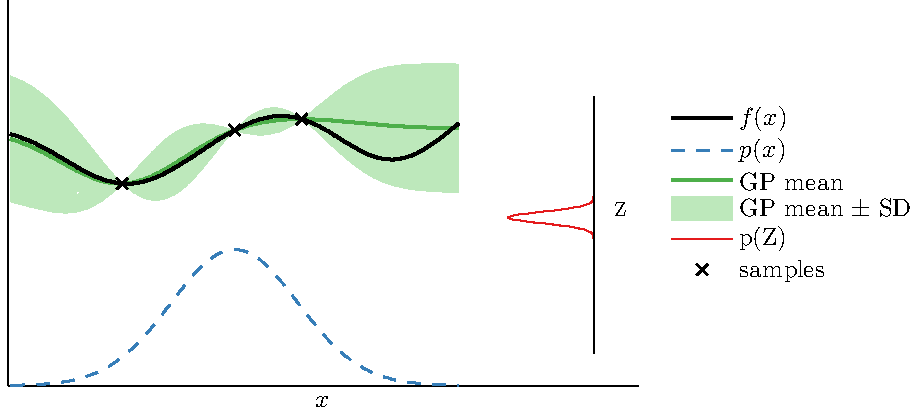
\includegraphics[width=11cm]{figures/bq_buildup/buildup_samps3}
\end{figure}



\section{The Link between MMD and GP Integrals}

[This section will show that the posterior variance of the difference between the integral of a GP with respect to two different distributions is equal to MMD.  This generalizes a result from \citep{huszar2012herdingbmcuai}]

\begin{prop} Given that $f$ is drawn from a standard GP prior, the expected squared difference in the integral between $f(x)$ against $p(x)$ minus the integral of $f(x)$ against $q(x)$ is equal to the squared Maximum Mean Discrepancy between $p$ and $q$.
\label{prop:gp_mmd}
\end{prop}
%
\begin{proof}
The proof involves invoking the representer theorem, using bilinearity of scalar products and the fact that if $f$ is a standard Gaussian process then $\forall g\in\He: \left\langle f,g\right\rangle \sim \mathcal{N}(0,\Hnorm{g}^2)$:
\begin{align}
%&\varianceargs{}{Z_{f,p}\vert f(x_1), \dots, f(x_N), x_1, \dots, x_N}=\\
%&\varianceargs{}{Z_{f,p}\vert x_1, \dots, x_N}=\\
	& \varianceargs{f\sim GP}{ \int f(x) p(x) dx -  \int f(x) q(x) dx }\\
	&= \mathbb{E}_{f\sim GP} \left( \int f(x) p(x) dx -  \int f(x) q(x) dx \right)^2\\
	&= \mathbb{E}_{f\sim GP} \left( \int \left\langle f, \phi (x)\right\rangle p(x) dx - \int \left\langle f, \phi (x)\right\rangle q(x) dx \right)^2\\
	&= \mathbb{E}_{f\sim GP} \left\langle f,  \int\phi(x) p(x) dx - \int\phi(x) q(x) dx \right\rangle^2\\
	&= \mathbb{E}_{f\sim GP} \left\langle f,  \mu_p - \mu_{q}\right\rangle^2\\	
	&= \Hnorm{\mu_p - \mu_q}^2\\
	&= \mmd^2(p,q)
\end{align}
\end{proof}


\subsection{Other links}

Energy distances and parzen window estimators. [Smola's talk]


\section{Kernel Herding and Bayesian Quadrature}

In this section we show that Bayesian Quadrature Kernel herding \citep{chen2010super}

\begin{prop} The expected variance in the Bayesian quadrature estimate $\epsilon^{2}_{\bq{}}$ is the maximum mean discrepancy between the target distribution $p(x)$ and $q_{\bq{}}(x) = \sum_{n=1}^{N}w^{(n)}_{\bq{}}\delta_{x_n}(x)$
\end{prop}
%
\begin{proof}
Because the true integral is $\int f(x) p(x) dx$ and the BQ estimator is given by $\sum_i f(x_i) w_{BQ}^{(i)}$,  Proposition \ref{prop:gp_mmd} implies that thier expected difference is given by $\mmd^2(p,q_{BQ})$.
\end{proof}

\subsection{Empirical estimator}

[Re-derive the empirical estimator]

\section{Kernel Two-sample Tests}

The kernel two-sample test was introducted by \cite{gretton2005kernel, gretton2008kernel}.  It was also proven [cite] that if $X \sim p, Y \sim q$, then $\mmd(X,Y)$ is an unbiased estimator of $\mmd(p,q)$.  Furthermore, the empirical MMD converges to the true MMD uniformly for any $p,q$.

related to Kernel ICA \cite{bach2003kernel}, which normalizes to lessen the effect of the marginals.

\begin{figure}
%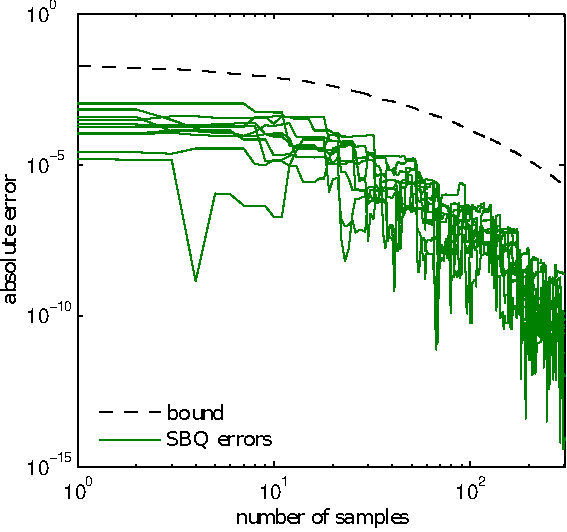
\includegraphics[width=\columnwidth]{figures/bound_curve_rkhs}
\caption{A graphical intepretation of the kernel two-sample test:  The test statistic measures expected difference in integrals between the two empirical distributions.}
\label{fig:ktst}
\end{figure}

\subsection{Bayesian Two-sample tests}

A Bayesian two-sample test was proposed by \cite{borgwardt2009bayesian}.  The nonparametric version of their test places Dirichlet process mixture of Gaussian priors on $p(x)$ and $q(x)$, and computes the Bayes factor comparing the hypotheses $\mathcal{H}_0 : p(x) = q(x)$ and  $\mathcal{H}_1 : p(x) \neq q(x)$.  This approach is appealing because it directly compares the likelihood of the two cases that two-sample tests are designed to compare.  However, the DP-MoG likelihood ratio cannot be computed in closed form.  

In comparison, the test statistic given by $\mmd(p,q)$ is an indirect measure by which to compare the two hypotheses of interest, but it does have a closed form solution.



\section{Hilbert-Schmidt Independence Criterion and GP Integrals}

New test statistic based on infinite-dimensional Frobenius norm of cross-covariance matrix of features of x and y: [Gretton et. al, 2005]
\begin{align}
\hsic(p(x,y),k_x, k_y) & = || C_{xy} ||^2_{HS}  \\
& = \expectargs{x, x', y, y'}{k_x(x,x')k_y(y,y)} + \expectargs{x, x'}{k_x(x,x')}\expectargs{y, y'}{k_y(y,y')} \\
\nonumber & \qquad - 2 \expectargs{x, y}{\expectargs{x'}{k_x(x,x')}\expectargs{y'}{k_y(y,y')}}
\end{align}


\begin{prop} The HSIC is equivalent to the variance in the squared difference of integrals of functions drawn from a GP prior against the joint distribution, and the product of the marginal distributions.
\end{prop}
%
\begin{proof}


We use the identities that for a zero-mean GP,

\begin{align}
\expectargs{f\sim \gp}{ f(x,y)} & = k(x,y) \\
\expectargs{f\sim \gp}{ f(x,x',y,y')} & = k(x,x',y,y')
\end{align}

\begin{align}
& \varianceargs{f\sim \gp}{ \int \!\!\! \int\!\! f(x,y)p_{xy}(x,y)dxdy - \int \!\!\! \int\!\! f(x',y')p_x(x')p_y(y')dx dy}\\
& = \expectargs{f\sim \gp}{ \left( \int \!\!\! \int\!\! f(x,y)p_{xy}(x,y)dxdy - \int \!\!\! \int\!\! f(x',y')p_x(x')p_y(y')dx dy \right)^2}\\
%
& = \expectargs{f\sim \gp}{ \int \!\!\! \int\!\! f(x,y)p_{xy}(x,y)dxdy \int \!\!\! \int\!\! f(x',y')p_{xy}(x',y')dx'dy'}\\
\nonumber & \qquad -2 \expectargs{f\sim \gp}{ \int \!\!\! \int\!\! f(x,y)p_{xy}(x,y)dxdy \int \!\!\! \int\!\! f(x',y')p_{x}(x')p_{y}(y')dx'dy'}\\
\nonumber & \qquad + \expectargs{f\sim \gp}{ \int \!\!\! \int\!\! f(x,y)p_{x}(x')p_{y}(y')dxdy \int \!\!\! \int\!\! f(x',y')p_{x}(x')p_{y}(y')dx'dy'}\\
%
& = \int \!\!\! \int \!\!\!\int \!\!\! \int\!\! k(x,x',y,y')p_{xy}(x,y)p_{xy}(x',y')dxdydx'dy' \\
\nonumber & \qquad + \int \!\!\! \int\!\!\! \int \!\!\! \int\!\! k(x,x',y,y') p_{x}(x)p_{x}(x')dxdx' p_y(y) p_y(y') dydy' \\
\nonumber & \qquad - 2 \int \!\!\! \int \!\!\!\int \!\!\! \int\!\! k(x,x',y,y') p_x(x') dx' p_y(y')dy p_x(x) p_y(y) dx dy \\
\end{align}
%
Then, using the assumption that $k(x,x',y,y') = k_x(x,x') k_y(y,y')$, we can continue:
%
\begin{align}
& = \int \!\!\! \int \!\!\!\int \!\!\! \int\!\! k_x(x,x')k_y(y,y')p_{xy}(x,y)p_{xy}(x',y')dxdydx'dy' \\
\nonumber & \qquad + \int \!\!\! \int\!\! k_x(x,x')p_{x}(x)p_{x}(x')dxdx'\int \!\!\! \int\!\! k_y(y,y') p_y(y) p_y(y') dydy' \\
\nonumber & \qquad - 2 \int \!\!\! \int\!\! \left[\int\!\! k_x(x,x') p_x(x') dx' \right]\left[\int\!\!k_y(y,y') p_y(y')dy\right] p_x(x) p_y(y) dx dy \\
%
& = \expectargs{x, x', y, y'}{k_x(x,x')k_y(y,y)} + \expectargs{x, x'}{k_x(x,x')}\expectargs{y, y'}{k_y(y,y')} \\
\nonumber  & \qquad - 2 \expectargs{x, y}{\expectargs{x'}{k_x(x,x')}\expectargs{y'}{k_y(y,y')}} \\
& = \hsic(p(x,y),k_x, k_y)	
\end{align}
\end{proof}

\subsection{Generalization of HSIC}

If we can come up with a more sensible kernel $k(x,x',y,y')$ than the factored kernel $k(x,x',y,y') = k_x(x,x') k_y(y,y')$, we obtain a more general solution:
%
\begin{align}
GHSIC & = \int \!\!\! \int \!\!\!\int \!\!\! \int\!\! k(x,x',y,y')p_{xy}(x,y)p_{xy}(x',y')dxdydx'dy' \\
\nonumber & \qquad + \int \!\!\! \int\!\!\! \int \!\!\! \int\!\! k(x,x',y,y') p_{x}(x)p_{x}(x')dxdx' k_y(y,y') p_y(y) p_y(y') dydy' \\
\nonumber & \qquad - 2 \int \!\!\! \int \!\!\!\int \!\!\! \int\!\! k(x,x',y,y') p_x(x') dx' p_y(y')dy p_x(x) p_y(y) dx dy \\
& = \expectargs{x, x', y, y'}{ k(x,x',y,y')p_{xy}(x,y)p_{xy}(x',y')} \\
\nonumber & \qquad + \expectargs{x, x', y, y'}{ k(x,x',y,y') p_{x}(x)p_{x}(x') p_y(y) p_y(y') } \\
\nonumber & \qquad - 2 \expectargs{x, x', y, y'} k(x,x',y,y') p_x(x') p_y(y') p_x(x) p_y(y)
\end{align}

\begin{figure}
%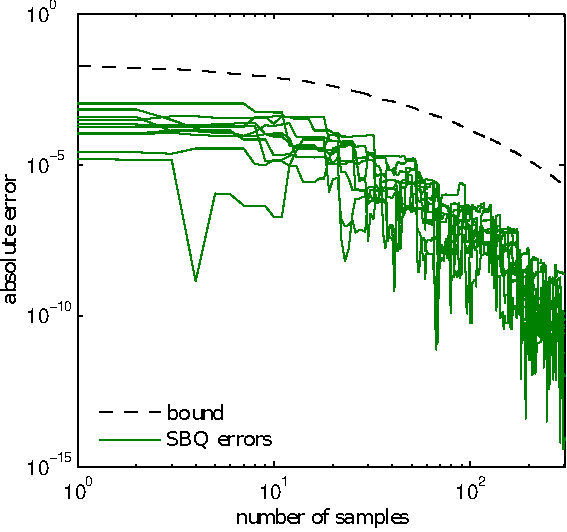
\includegraphics[width=\columnwidth]{figures/bound_curve_rkhs}
\caption{A graphical intepretation of the HSIC:  The expected difference in integrals under the joint empirical distribution, and the product of marginal empirical distributions.}
\label{fig:hsic}
\end{figure}

\subsection{Empirical estimator}

The empricial estimate of HSIC is given by:

\begin{align}
\vectornorm{\hat{\Sigma}^{(N)}_{YX}}^2_{HS} = \frac{1}{N^2}
\end{align}


\section{Mean Embeddings and Conditional Mean Embeddings}

Many results in the MMD literature discuss the \emph{mean embedding} of a distribution in a RKHS.  What is the corresponding Bayesian intepretation?  Based on a result due to \cite{krikproof}, we can say that if $f \sim \gp$,
%
\begin{align}
\mu_{p(x)} 	& = \int \! \phi(x) p(x) dx \\
		   	& = \int \! k(x, \cdot) p(x) dx \\
			& = \expectargs{f \sim \gp}{ \int \!\! f(x) f(\cdot) p(x) dx} \\
			& = \expectargs{f \sim \gp}{ f(\cdot) \int \!\! f(x) p(x) dx}			
	%		& = \int \!\!\! \int \!\! f(x) f(\cdot) p(x) dx \gp \left( f | \vzero, k(x, x') \right) df
\end{align}
%
Thus we can interpret the mean embedding of $p(x)$ as the expected covariance of each point of the function with its integral with respect to $p(x)$.
%For characteristic kernels [cite], the mean embedding fully characterizes the distribution.


\section{Kernel Conditional Independence Tests}

Kernel Conditional Independence Tests \cite{fukumizu2008kernel}

Cross-covariance operator is defined as:Proposition \ref{prop:gp_mmd}
\begin{align}
\left\langle f, \Sigma_{YX} g\right\rangle = \cov[f(X), g(Y)] = \expect{f(X)g(Y)} - \expect{f(X)} \expect{g(Y)}
\end{align}

Normalized conditional cross-covariance operator:

\begin{align}
V_{YX|Z} = V_{YZ} V_{ZX}
\end{align}

conditional covariance operator:
\begin{align}
\Sigma_{YX|Z} = \Sigma_{YX} - \Sigma_{YZ} \Sigma_{ZZ}\inv \Sigma_{ZX}
\end{align}

Attempted interpretation of the unnormalized version of their test:

\begin{align}
I^{CONDU} & = \varianceargs{f\sim \gp}{ \int \!\!\! \int\!\! f(x,y, z, z')p_{xy}(x,y|z)dxdy - \int \!\!\! \int\!\! f(x',y')p_x(x'|z)p_y(y'|z)dx dy} \\
& = \expectargs{z\sim p(z)}{\mmd( p_{xy}(x,y|z)dxdy, p_x(x'|z)p_y(y'|z)} \\
\end{align}



We should probably think of conditional independence given $z$ as a function of $z$, but we can summarize this function by its expectation.

The naive test is identically zero under the empirical distribution:
\begin{align}
BCIT_1 & = \expectargs{z\sim p(z)}{\varianceargs{f\sim \gp}{ \int \!\!\! \int\!\! f(x,y)p_{xy}(x,y|z)dxdy - \int \!\!\! \int\!\! f(x',y')p_x(x'|z)p_y(y'|z)dx dy}} \\
& = \expectargs{z\sim p(z)}{\mmd( p_{xy}(x,y|z)dxdy, p_x(x'|z)p_y(y'|z)} \\
& = \frac{1}{N} \sum_i \int \!\!\! \int \!\!\!\int \!\!\! \int\!\! k(x,x',y,y',z,z)p(x,y|z)p(x',y'|z)dxdydx'dy' \\
\nonumber & \qquad + \int \!\!\! \int\!\!\! \int \!\!\! \int\!\! k(x,x',y,y',z,z) p(x|z)p(x'|z)dxdx' p(y|z) p(y'|z) dydy' \\
\nonumber & \qquad - 2 \int \!\!\! \int \!\!\!\int \!\!\! \int\!\! k(x,x',y,y',z,z) p(x'|z) dx' p(y'|z)dy p(x|z) p(y|z) dx dy \\
& = 0
\end{align}
using the empirical distribution for $p(x,y|z)$, which will be multiplied by zero whenever $p(z) = 0$.


\subsection{Bayesian Interpretation of HS norm}

The HS-Norm of operator $A$ is given by $||A||_{HS}^2 = \sum_i,j \left\langle \psi_j, A \phi_i \right\rangle^2_{\mathcal{H}_2}$.


\section{Related Work}

The MMD has been related to energy distances \cite{sejdinovic2012hypothesis, sejdinovic2012equivalence}, proving that energy distances [define] are equivalent to MMD.  Thus, we can claim as a corollary of Proposition \ref{prop:gp_mmd} that energy distances are also equivalent to the variance of difference of integrals.

\section{Open Questions}

Can the Bayesian interpretation be extended to covariate shift?

What is the intepretation of normalization in the kernel conditional dependence work?

Instead of low-rank approximation, can we use other sparse GP methods?

\section{Applications}

\subsection{Semi-supervised classification or ICA}

We can learn the kernel such that the empirical distribution of labeled examples from the same class are forced to be together, and those from different classes are forced to be apart.  Can we then interpret $f$, the function drawn from the GP prior?  Would $f$ then be the "class membership" function?

\subsection{The witness function}

Does the witness function have a Bayesian interpretation?  It equals $w(x') = \int (p(x)-q(x)) k(x, x') dx$, which is the difference between p and q convolved with the kernel function.


\begin{align}
%&\varianceargs{}{Z_{f,p}\vert f(x_1), \dots, f(x_N), x_1, \dots, x_N}=\\
%&\varianceargs{}{Z_{f,p}\vert x_1, \dots, x_N}=\\
 & \mmd^2(p,q) \\
	&= \varianceargs{f\sim GP}{ \int f(x) p(x) dx -  \int f(x) q(x) dx }\\
	&= \varianceargs{f\sim GP}{ \int f(x) \left[ p(x) -q(x) \right] dx}\\
	&= \expectargs{f\sim GP}{ \left(\int f(x) \left[ p(x) -q(x) \right] dx \right)^2}\\	
	&= \expectargs{f\sim GP}{ \left(\int f(x) \left[ p(x) -q(x) \right] dx \right)\left(\int f(x') \left[ p(x') -q(x') \right] dx' \right)}\\	
	&= \expectargs{f\sim GP}{ \int \int f(x) f(x') \left[ p(x) -q(x) \right] \left[ p(x') -q(x') \right] dx dx' }\\	
	&=  \int \int k(x,x') \left[ p(x) -q(x) \right] \left[ p(x') -q(x') \right] dx dx'\\
	&=  \int w(x) \left[ p(x') -q(x') \right] dx'
\end{align}
%
So, the expectation of the witness function is the MMD.



\section{Summary}
\begin{table}[h]
\caption{Almost-equivalent Methods}
\label{sample-table}
\begin{center}
\begin{tabular}{llll}
\multicolumn{2}{c}{ \bf Frequentist Method}  &\multicolumn{2}{c}{\bf Bayesian Method}
\\ \hline \\
$\mathcal{O}(N^2)$ & Kernel herding        					& $\mathcal{O}(N^3)$ & Bayesian Quadrature \\
$\mathcal{O}(N^2)$ & Hilbert-Schmidt Independence Criterion & $\mathcal{O}(N^3)$ & Variance of difference of integrals \\
$\mathcal{O}(N^2)$ & Kernel Two-sample test				    & $\mathcal{O}(N^3)$ & Variance of difference of integrals
\end{tabular}
\end{center}
\end{table}


\begin{table}[h]
\caption{Related Methods}
\label{sample-table}
\begin{center}
\begin{tabular}{llll}
\multicolumn{1}{c}{ \bf Frequentist Method}  &\multicolumn{1}{c}{\bf Bayesian Method}
\\ \hline \\
Kernel Regression (Nadayara-Watson)			& GP Regression \\
Functional ANOVA, HKL						& Additive Gaussian Processes \\
Kernel Bayes' Rule							& Bayesian Quadrature for Ratios \\
Conditional Mean Embeddings 				& Gaussian Process Dynamic Programming \\
Kernel Message Passing 						& ???
\end{tabular}
\end{center}
\end{table}




\subsubsection*{Acknowledgments}

We would like to thank Miguel Hernandez-Labato, Roger Grosse, Philipp Hennig, and Michael Osborne for helpful suggestions and advice.

\bibliographystyle{style/icml2013}
\bibliography{connections}

\end{document}

